\section{Interfaz 3.00 Selección de nivel}\label{inter:interfaz03}
	\subsection{Descripción de la pantalla}
Muestra el nombre de la pantalla en la esquina superior izquierda.
Los iconos de nivel y de las cinemáticas estarán organizados en un carrusel que permitirá su selección. Los niveles y cinemáticas disponibles a elegir en el carrusel dependerán de la carga automática. Los niveles disponibles disponibles para jugar mostrarán una imagen descriptiva en el carrusel mientras que los niveles no disponibles mostraran un imagen de un cuadro negro.   
Bajo el carrusel se encontrara un apartado donde se podrá visualizar información del nivel seleccionado en el carrusel, tal como el nombre y una breve descripción.
El botón que permite iniciar una partida en el nivel seleccionado se encontrará ubicado al lado derecho de la sección donde se muestra la información del nivel. 
	\subsection{Estados del juego}
Se llega a esta interfaz a través de la interfaz 2.00 (ver apartado\ref{inter:interfaz02}), siempre que el Jugador oprima el botón de cargar partida.
La interfaz 3.0 cuenta con los siguientes botones:
\begin{itemize}
	\item \textbf{Iniciar Nivel}: Envía al inicio del nivel seleccionado.
	\item \textbf{Control de carrusel}: estos botones permite controlas los elementos que se almacenan en el carrusel.
\end{itemize} 
	\subsection{Imagen}
	Ver figura \ref{fig:SelNivel}
\begin{figure}
  \centering
   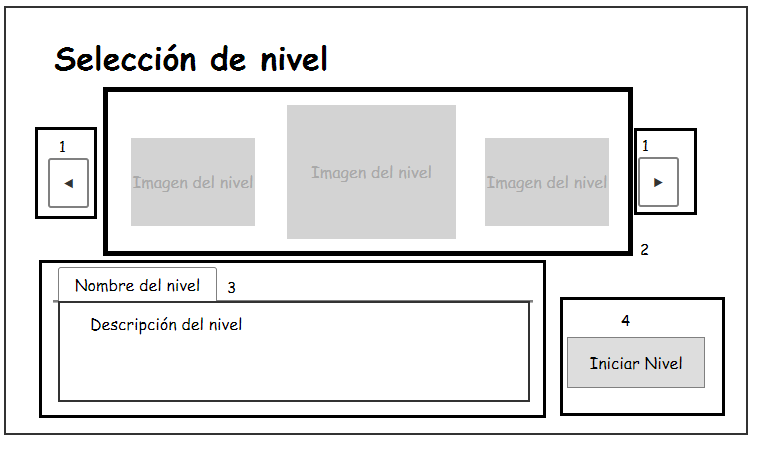
\includegraphics[width=0.6 \textwidth]{Imagenes/interfaz02_01}
  \caption{Interfaz 2.00 Selección de nivel.1 botones que controlan el carrusel. 2 Carrusel. 3 Información del nivel seleccionado. 4 Botón Iniciar nivel.}
  \label{fig:SelNivel}
\end{figure} 